\section{Emergence, Benefits and Limitations of Using Edge Computing}

\begin{table*}[t]
\caption{Edge Computing use cases, current limitations, and imperatives}
\label{tab:use_case}
\begin{tabular}{|c|c|c|c|}
\hline
Applications                  & Example Use Case                                                                                                                                                                     & Limitations                                                                                                                                                      & Requirements                                                                                                                                       \\ \hline
Smart City                & \begin{tabular}[c]{@{}c@{}}Help autistic people \\ navigate through large \\ crowded spaces.\end{tabular}                                                                        & \begin{tabular}[c]{@{}c@{}}Hard to provide real-time \\ directions due to the need to \\ send large volumes of data to \\ the cloud.\end{tabular}                & \begin{tabular}[c]{@{}c@{}}Low Latency, Security,\\ Geographically \\ Distributed,\\ Mobility, Scalability\\ Reliability and Robustness\end{tabular} \\ \hline
\begin{tabular}[c]{@{}c@{}}Disaster \\ Recovery\end{tabular}        & \begin{tabular}[c]{@{}c@{}}Need to quickly determine \\ whether  building conditions \\ are safe for  evacuees to return \\ after a natural  disaster \\ has struck.\end{tabular} & \begin{tabular}[c]{@{}c@{}}Hard to perform real-time \\ decision due to the need to \\ send large volumes of data to \\ the cloud.\end{tabular}                  & \begin{tabular}[c]{@{}c@{}}Low Latency,\\ Geographically  \\ Distributed,\\ Orchestration \\ and Management\end{tabular}                                 \\ \hline
\begin{tabular}[c]{@{}c@{}}Distributed \\ Observatories\end{tabular} & \begin{tabular}[c]{@{}c@{}}Large networked system of \\ under water instruments \\ to collect real-time data \\ from the ocean.\end{tabular}                                   & \begin{tabular}[c]{@{}c@{}}Hard to deliver near \\ real-time data to the end user \\ due to the need to send large\\  volumes of data to the cloud.\end{tabular} & \begin{tabular}[c]{@{}c@{}}Low Latency, Security,\\ Geographically \\ Distributed,\\ Multi-Tenancy, Scalability\end{tabular}                         \\ \hline
\begin{tabular}[c]{@{}c@{}}Video \\ Analaytics\end{tabular}          & \begin{tabular}[c]{@{}c@{}}Video analytics for safety \\ and security from public \\ video cameras.\end{tabular}                                                                & \begin{tabular}[c]{@{}c@{}}Hard to perform real-time \\ analytics due to the need to \\ send large volumes of data to \\ the cloud.\end{tabular}                 & \begin{tabular}[c]{@{}c@{}}Low Latency, Security,\\ Geographically \\ Distributed,\\ Scalability\end{tabular}                                        \\ \hline
\end{tabular}
\end{table*}


\section{Motivating Applications}\label{sec:usecases} 
IoT applications are present in several domains: Precision medicine, Urban mobility, and Healthcare.
In this section, we highlight four different use cases described in both industry and academia that benefits from the IoT paradigm. 
Table~\ref{tab:use_case} summarises the scenario, limitations and requirements of those use cases.

%To better understand the need for an edge middleware, this section presents four scenarios to motivate the need.

\subsection{Smart City}

The first use case is smart cities for people with disabilities. Large cities are difficult to navigate, especially for people with special needs such as those with visual impairment, Autism Spectrum Disorder (ASD), or simply those with navigational challenges. The primary objective of this application use case is to explore the use of IoT capabilities to transform cities around the world into smart cities capable of providing location-aware services (e.g., finding buildings and streets, improving travel experience, obtaining security alerts). In order to create smart cities that can support reliable navigation services to people with special needs, researchers are creating complex workflows integrating a number of novel IoT elements, including video analytics, Bluetooth beacons, mobile computing, and LiDAR-scanned 3D semantic models. For example, we may have a streaming application workflow that analyzes video feeds from the surveillance cameras of the streets in real-time to evaluate the density of crowds in different parts of the city to help select path choices. Especially, ASD individuals may prefer to choose paths that have less dense crowds due to psychological factors; people with visual impairment try to avoid large open spaces due to the difficulty of finding references for localization, and people in wheelchairs can navigate along paths with fewer crowds far more conveniently than among those with large crowds. This information is then combined with a 3D model and the location of the user to calculate the best path to reach the desired destination. Additionally, we need to continuously monitor the user (e.g., using the Bluetooth beacons), and the streets (e.g., using surveillance cameras) to adapt to changes. In the smart city use case, since there are multiple video cameras in different locations, sending the video feeds of this camera to the cloud will incur high latencies, bandwidth congestions, and privacy concerns.

\subsection{Disaster Recovery}

Our second use case is a disaster response use case. Disaster management is a process that involves four phases: mitigation, preparedness, response, and recovery. Mitigation efforts attempt to prevent hazards from developing into disasters altogether or to reduce the effects of disasters when they occur. In the preparedness phase, emergency managers develop plans of action when the disaster strikes and analyze and manage the required resources. The response phase executes the action plans, which include the mobilization of the necessary emergency services and dispatch of first responders and other material resources in the disaster area. Finally, the aim of the recovery phase is to restore the affected area to its previous state. This workflow focuses on the response phase by using a multi-stage generic response workflow that will be executed at the edge and at the core of the network. The workflow starts by capturing real-time data of the affected zones (e.g LiDAR, photogrammetry, etc.) and we perform a pre-processing stage at the edge of the network. In our case, a minivan or a drone with networking and computational capabilities will be used to determine the content of the data and if any further post-processing is needed. If further processing is needed, data will be either sent to the cloud to perform a change detection with previously recorded historical data, store data into the cloud, or notify agencies to determine if building conditions are safe. In the disaster recovery use case, the mapping of an affected area can have a total of 741 images and total 3.7 GB, with the biggest image 33.8 MB and the smallest 1.8 KB, taking over 1 hour to transfer all the data to the cloud with a 4G connection.

\begin{figure}[ht]
  \centering
  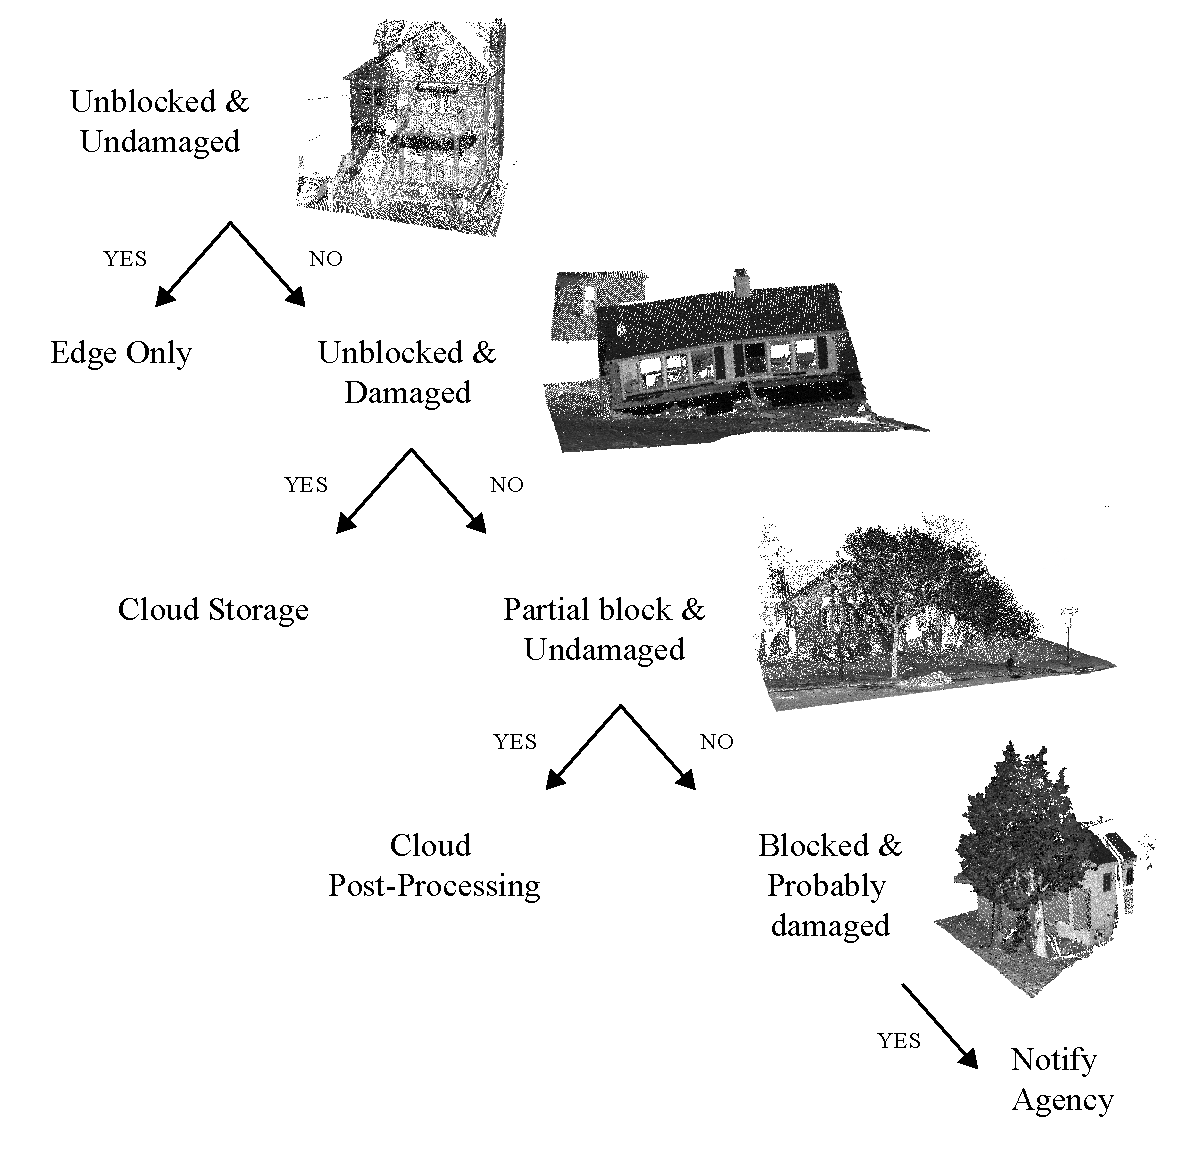
\includegraphics[width=0.5\linewidth]{Figures/diagonal.pdf}
  \caption{Disaster recovery decision stages and its associated reactions based on the LiDAR images.}
  \label{data_uncertainty}
\end{figure}

\subsection{Scientific Observatory}

It's a networked ocean research observatory with arrays of instrumented water column moorings and buoys, profilers, gliders, and autonomous underwater vehicles within the different open ocean and coastal regions. OOI infrastructure also includes a cabled array of instrumented seafloor platforms and water column moorings on the Juan de Fuca tectonic plate. This networked system of instruments, moored and mobile platforms, and arrays provide ocean scientists, educators, and the public the means to collect sustained, time-series data sets to enable the examination of complex, interlinked physical, chemical, biological, and geological processes operating throughout the coastal regions and open ocean. OOI implements a geographically distributed, secure, highly available CI that is responsible for data acquisition/collection, data storage and processing, and on-demand delivery of data and data products to scientists and application developers. The use of a well-defined API based on standard protocols enables other systems to interface and interact with OOI CI programmatically. The scientific observatory use case has a similar problem to the disaster recovery use case where the data is to big to send to the cloud in order to offer real-time data delivery.

\subsection{Video Analytics} 

The last use case is the use of video analytics~\cite{8358733} for safety and security. In video analytics, a single video camera can produce about 25-30 frames/second. In HD and FHD cameras an 8-bit uncompressed RGB frame amounts to about 553 Mbps and 1.24 Gbps for a one minute video, respectively. With the advent of 4k and 3D video cameras, this size is likely to grow exponentially. Developers and engineers are facing the challenge of providing on-time analytics of video data to support public safety and security from video cameras. Cloud computing is not efficient enough to support prompt analytics of such video data~\cite{7488250}. Video Analytics based on edge computing is the only feasible approach to cater to low latency requirement for large-scale video streams~\cite{8057318}.

\subsection{Observe Orient Decide Act Loop}

The \ac{OODA} loop refers to the decision-making cycle of observe, orient, decide, and act, developed by military strategists and the United States Air Force~\cite{OODA}. \ac{OODA} is a decision-making cycle to process data streaming from sensors in real time, becoming an essential design characteristic for IoT applications. 
\begin{figure}[h!]
  \centering
  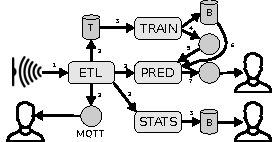
\includegraphics[width=0.8\columnwidth]{Figures/ooda.pdf}
  \caption{RIoTBench IoT high-level logical interactions between different sensors, applications and users.}
  \label{fig:etl}
\end{figure}

Anshu \textit{et al.}~\cite{RIoTBench} offer a suite of IoT applications that follows the closed-loop \ac{OODA} cycle. The applications are based on common IoT patterns for data pre-processing, statistical summarization, and predictive analytics. These are coupled with workloads sourced from real IoT observations. A high-level overview of the logical interaction of the IoT applications is depicted in Figure~\ref{fig:etl}.

\textbf{Extract-Transform-Load (ETL)} consumes data from hundreds of thousands of edge sensors, and pre-processes, cleans, and archives the data. Further, the results are published to an edge broker so that clients interested in real-time monitoring can subscribe to it, while a copy is forked to the cloud for storage, and another to the next dataflow step.

\textbf{Statistical Summarization (STATS)} performs higher order aggregation and plotting operations, and stores the generated plots into the cloud, from where webpages can load the visualization files on browsers. 

\textbf{Model Training (TRAIN)} periodically loads the stored data from ETL step and trains forecasting models that are stored in the cloud, and notifies the message broker of an updated model being available. 

\textbf{The Predictive Analytics (PRED)} subscribe to the message broker and downloads the new models from the cloud, and continuously operates over the pre-processed data stream from ETL to make predictions and classifications that can indicate actions to be taken on the domain. It then notifies the message broker of the predictions, which can independently be subscribed to by a user or device for action. 

The ETL dataflow requires a low-latency cycle in order to achieve real-time monitoring, in addition it also requires some of its operators to be located in the cloud for storing messages and others to be at the edge of the network. This makes the ETL workflow the perfect candidate workflow for testing the operator placement strategy proposed. 